\subsection{Space-Time Diagrams}
Consider one spatial dimension \(x\) and one temporal dimention \(t\) in an inertial frame \(S\).
We can plot \(x\) on the horizontal axis and \(ct\) on the vertical axis, in order to make the units match.
This combination of space and time in one diagram is called Minkowski spacetime.
Each point \(P\) in spacetime represents an event labelled by coordinates \((x, ct)\).
A moving particle traces out a curve in this diagram, called the world line.
\begin{center}
	\begin{tikzpicture}
		\begin{axis}[
				axis lines = left,
				xlabel = \(x\),
				ylabel = \(ct\),
				xtick=\empty,
				ytick=\empty,
			]

			\fill (axis cs:2,1) circle[radius=2pt];
			\node[anchor=south] at (axis cs:2,1) {\(P\)};

			\addplot[domain=0:3, samples=500] {0.5*x + 0.03*sin(deg((pi * x)^(1.5)))};
		\end{axis}
	\end{tikzpicture}
\end{center}
The world line would be a straight line if the particle is moving at a constant velocity.
In particular, light rays have gradient 1.
Since particles cannot travel faster than the speed of light, world lines are restricted to certain regions (drawn in red) of the space time plane, given that the particle is at \(x=0\) when \(t=0\).
\begin{center}
	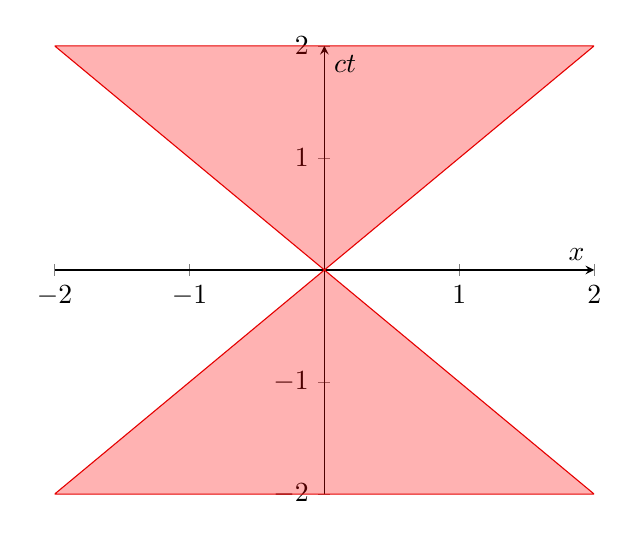
\begin{tikzpicture}
		\begin{axis}[
				axis lines = center,
				xlabel = \(x\),
				ylabel = \(ct\),
			]

			\addplot [red!90!black, fill=red, fill opacity=0.3] coordinates {
					(0, 0) (2, 2) (-2, 2) (2, -2) (-2, -2)
				} -- cycle;
		\end{axis}
	\end{tikzpicture}
\end{center}
We can also draw the axes of a different frame \(S'\) on the same diagram, moving at speed \(v\) relative to \(S\).
The \(t'\) axis corresponds to the equation \(x'=0\) and therefore corresponds to \(x=vt\), or equivalently \(x = \frac{v}{c} \cdot ct\).
The \(x'\) axis corresponds to \(t'=0\), which is \(ct = \frac{v}{c}\cdot x\).
\begin{center}
	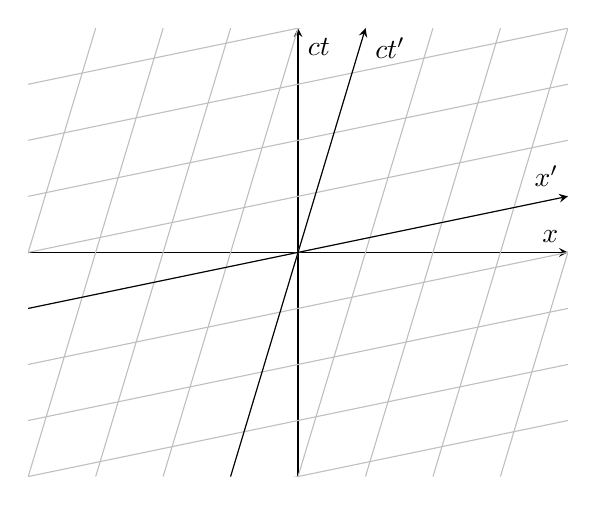
\begin{tikzpicture}
		\begin{axis}[
				axis lines = center,
				xlabel = \(x\),
				ylabel = \(ct\),
				xmin=-2,
				ymin=-2,
				xmax=2,
				ymax=2,
				xtick=\empty,
				ytick=\empty,
			]

			\draw[color=lightgray] (axis cs: -2.5, -2) -- (axis cs: -1.5, 2);
			\draw[color=lightgray] (axis cs: -2, -2) -- (axis cs: -1, 2);
			\draw[color=lightgray] (axis cs: -1.5, -2) -- (axis cs: -0.5, 2);
			\draw[color=lightgray] (axis cs: -1, -2) -- (axis cs: 0, 2);
			\draw[color=lightgray] (axis cs: -0.5, -2) -- (axis cs: 0.5, 2);
			\draw[color=lightgray] (axis cs: 0, -2) -- (axis cs: 1, 2);
			\draw[color=lightgray] (axis cs: 0.5, -2) -- (axis cs: 1.5, 2);
			\draw[color=lightgray] (axis cs: 1, -2) -- (axis cs: 2, 2);
			\draw[color=lightgray] (axis cs: 1.5, -2) -- (axis cs: 2.5, 2);

			\draw[color=lightgray] (axis cs: -2, -2.5) -- (axis cs: 2, -1.5);
			\draw[color=lightgray] (axis cs: -2, -2) -- (axis cs: 2, -1);
			\draw[color=lightgray] (axis cs: -2, -1.5) -- (axis cs: 2, -0.5);
			\draw[color=lightgray] (axis cs: -2, -1) -- (axis cs: 2, 0);
			\draw[color=lightgray] (axis cs: -2, -0.5) -- (axis cs: 2, 0.5);
			\draw[color=lightgray] (axis cs: -2, 0) -- (axis cs: 2, 1);
			\draw[color=lightgray] (axis cs: -2, 0.5) -- (axis cs: 2, 1.5);
			\draw[color=lightgray] (axis cs: -2, 1) -- (axis cs: 2, 2);
			\draw[color=lightgray] (axis cs: -2, 1.5) -- (axis cs: 2, 2.5);

			\draw[->,>=stealth] (axis cs: -0.5, -2) -- (axis cs: 0.5, 2);
			\node[anchor=north west] at (axis cs:0.5,2) {\(ct'\)};
			\draw[->,>=stealth] (axis cs: -2, -0.5) -- (axis cs: 2, 0.5);
			\node[anchor=south east] at (axis cs:2,0.5) {\(x'\)};

		\end{axis}
	\end{tikzpicture}
\end{center}
The angle between the \(x\) and \(x'\) axes matches the angle between the \(ct\) and \(ct'\) axes; they are symmetric about the diagonal (as are the original \(x\) and \(ct\) axes).
Note that the diagonal is given by \(x=ct\) and \(x'=ct'\), which is the same light ray.

\subsection{Comparing Velocities}
Conside ra particle moving with constant velocity \(u'\) in \(S'\), where \(S'\) is travelling at velocity \(V\) with respect to \(S\).
The world line of the particle in \(S'\) is simply \(x' = u' t'\).
Correspondingly in \(S\), \(x=ut\).
Now, using the Lorentz transformation,
\[
	x=\gamma(x' + vt') = \gamma(u' + v)t'
\]
\[
	t = \gamma\qty(t' + \frac{vx'}{c^2}) = \gamma\qty(1 + \frac{vu'}{c^2})t'
\]
Hence,
\[
	u = \frac{x}{t} = \frac{u' + v}{1 + \frac{u'v}{c^2}}
\]
Note that
\[
	c-u = \frac{(c - u')(c - v)}{1 + \frac{u' v}{c^2}}
\]
which is always positive if \(u'<c\) and \(v<c\).
Therefore, a Lorentz transformation preserves the property that a speed is smaller than the speed of light.

\subsection{Simultaneity}
Two events \(P_1\) and \(P_2\) are simultaneous in \(S\) if they occur at the same time in \(S\).
This is a line parallel to the space axis in the spacetime diagram.
In another reference frame, this line of constant time might be at a different angle.
So events simultaneous in \(S'\) may not correspond to events simultaneous in \(S\).
We can use the above formulae to deduce the exact time that an event happens in a different frame of reference.

\subsection{Causality}
Different observers may disagree on the time ordering of events, but we can construct a viewpoint which gives a consistent description of `cause' and `effect', so special relativity does not break causality.
Note that lines of simultaneity cannot have an angle greater than \(\frac{\pi}{2}\) since the speed of the moving frame must be less than \(c\).
We can construct a `light cone' from all lines or surfaces from an event \(P\) at an angle \(\frac{\pi}{2}\) to the time axis, which represents the possible effects of an event.
\begin{center}
	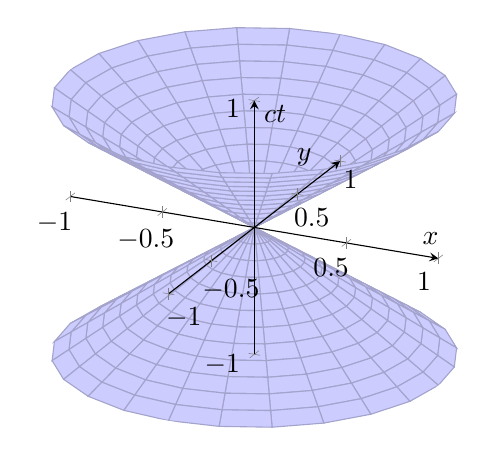
\begin{tikzpicture}
		\begin{axis}[
				axis lines=center,
				axis on top,
				%plot box ratio=1 1 1,
				xlabel=\(x\),
				ylabel=\(y\),
				zlabel={\(ct\)},
				%shader=flat,
				colormap={blue}{rgb=(0.8,0.8,1.0) rgb=(0.8,0.8,1.0)}
			]
			\addplot3 [surf, domain=-1:1, y domain=0:2*pi, z buffer=sort, colormap name=blue] ({x*cos(deg(y))},{x*sin(deg(y))},{x});
		\end{axis}
	\end{tikzpicture}
\end{center}
The cone above the origin is the `future light cone' and the cone below is called the `past light cone'.
Note that this cone is fixed under Lorentz transformations.
If an event occurs in the future light cone, then all observers agree that this event occurs after that the event at the origin.
Likewise, if an event occurs in the past light cone, all observers agree that this event occurs before the event at the origin.
Note that if an event \(P\) is not in the light cone, then it cannot cause, or be caused by, the event at the origin, since nothing travels faster than \(c\).
Hence, an event at the origin can only be influenced by events inside the past light cone, and may only influence events inside the future light cone.

\subsection{Time Dilation}
Consider first a clock which is stationary in \(S'\), which ticks at constant intervals \(\Delta t'\).
What is the time interval between ticks as perceived in \(S\)? We can use the Lorentz transformation, noting that \(x'=0\) since the clock is stationary in \(S'\), to get
\[
	t = \gamma\qty(t' + \frac{vx'}{c^2}) = \gamma t'
\]
Hence,
\[
	\Delta t = \gamma \Delta t'
\]
So moving clocks run slowly.
